\chapter{Mutation Pipeline QC}
\label{chap:mut-pipeline-qc}

% Somatic mutation QC report (2018.08)
% https://docs.google.com/document/d/1LW7HBKTwjz3-WCx0j2UedFPSVauulYom2qCbUW3Czbw/edit
% Somatic mutation QC Manuscript (2018.12)
% https://docs.google.com/document/d/1lObJXoxlM4t35DfRjGdZ_xJh3d59VuV7b7B1nGwIuy0/edit

\section{Summary}
We present a systematic analysis of the effects of synchronizing a large-scale, deeply characterized, multi-omic dataset to the current human reference genome, using updated software, pipelines, and annotations.
For each of 5 molecular data platforms in The Cancer Genome Atlas (TCGA)---mRNA and miRNA expression, single nucleotide variants, DNA methylation and copy number alterations---comprehensive sample, gene, and probe-level studies were performed, towards quantifying the degree of similarity between the \enquote*{legacy} GRCh37 (hg19) TCGA data and its GRCh38 (hg38) version as \enquote*{harmonized} by the Genomic Data Commons.
We offer gene lists to elucidate differences that remained after controlling for confounders, and strategies to mitigate their impact on biological interpretation.
Our results demonstrate that the hg19 and hg38 TCGA datasets are very highly concordant, promote informed use of either legacy or harmonized omics data, and provide a rubric that encourages similar comparisons as new data emerge and reference data evolve.


\section{Introduction}
Over the course of a decade The Cancer Genome Atlas (TCGA) helped usher in the era of extreme-scale team science, yielding numerous biological insights and many widely cited papers \cite{hutterc_zenklusenjc:CancerGenome2018}. Underlying this progress in understanding the molecular bases of cancer is one of the broadest, deepest, and most integratively characterized biological datasets ever assembled: on the order of 2 petabytes of primary and secondary data, in the form of 84,000 data aliquots from some 11,300 patients across 33 disease studies. Most TCGA samples were originally aligned against the Genome Reference Consortium build GRCh37 (hg19), with a small fraction (from the pilot phase of TCGA) having been aligned against NCBI Build 36.1 (hg18). Since TCGA was initiated, however, the research community has undergone tremendous evolution, not only in the characterization machinery, due to the enormous drop in sequencing costs, but also in the surrounding ecosystem of reference data, sequence alignment methods, variant calling tools, RNA quantification methods, quality controls used to help distinguish signal from noise, and analysis software. For this reason, the Genomic Data Commons (GDC, \url{https://gdc.cancer.gov/}) was conceived by the National Cancer Institute (NCI) as more than just a massive warehouse of digitized samples: instead, by harmonizing those samples to a uniform reference alignment and gene annotation, then characterizing samples with established tools in consistent workflows and providing updates at regular intervals, the GDC also helps navigate an orderly course through this sea of constant change. The GDC thus offers promise as a force-multiplier for researchers, who can now spend more time exploring their biological questions and less on resolving inconsistencies in data and software versions.

In this paper, we examine the results of the first major harmonization effort undertaken at the GDC: in which the corpus of legacy TCGA data was either aligned or lifted over to the GRCh38 build (hg38) with a GDC workflow assembled from updated versions of bioinformatic tools and reference files used by sequencing and characterization centers in TCGA. While the mechanics of evaluation varied for each data platform, owing largely to natural differences between them and/or how their hg19 counterparts were harmonized to hg38 (e.g., re-alignment of single nucleotide variants [SNVs] versus liftover of SNP6 copy number arrays), in each case \enquote{the aim was to categorize observed differences in analytic results as a function of their sources and control for such to discern potential impact upon biological interpretation.} The sources of variation are given in a figure for each platform and include, among others: (1) genome reference; (2) gene annotation: e.g. UCSC genes, GENCODE, miRBase; (3) upstream methods used in alignment, variant calling and quantification, including: BWA \cite{lih_durbinr:BWAShortRead2009}, STAR \cite{dobina_gingerastr:STARUltrafast2013}, RSEM \cite{lib_deweycn:RSEMAccurate2011}, FPKM-HTSeq \cite{anderss_huberw:HTSeqPython2015}, and MuTect \cite{cibulskisk_getzg:SensitiveDetection2013}; (4) downstream methods used in clustering, correlation, or significance analysis, such as GISTIC \cite{mermelch_getzg:GISTIC2Facilitates2011}; (5) parameterizations such as: thresholds for filtering, p-values or q-values; and (6) auxiliary data, such as: GISTIC marker files and CNV lists, or panels of normals used to remove suspect SNVs. In the interest of reproducibility, the supplement describes the software codes and parameterizations used to carry out these studies, and for each platform includes manifests of the input files upon which our analyses were executed. In the remainder of the text we use the terms ``legacy data'' and ``harmonized data'' interchangeably with ``hg19 data'' and ``hg38 data'', respectively.


\section{Results}

\subsection{Somatic Mutations}
TCGA somatic mutation data were generated by whole-exome sequencing in which exome capture was performed using the Agilent SureSelect Human All Exon kit. During TCGA, multiple sequencing platforms (Illumina and SOLiD) were employed. As described in Figure 5A, the analysis pipeline for calling hg38 somatic mutations at the GDC differs substantially from that for calling hg19 somatic mutations in TCGA legacy version (i.e., multi-Center Mutation Calling in Multiple Cancers; MC3 \cite{ellrottk_tcga:MC3MutationCalling2018}).
Although both pipelines used a multiple-caller strategy, there are still some differences---in the processing of alignment files, versions of mutation callers, mutation filters, and gene annotations (\fref{fig:mut-call-qc-pipeline-comparison})---between the MC3 (hg19) and GDC (hg38) mutations.
To characterize those differences and evaluate concordance with prior results, we compared the public somatic mutation calling of single nucleotide variations (SNVs) on multiple TCGA cohorts, using 2,069 samples from the breast, leukemia, colorectal and ovarian cancer cohorts (BRCA, LAML, COAD and OV). We also investigated the `protected' somatic mutation calls of the two groups, which represented the pre-filtered calls. A protected call was excluded from the public call set if it was considered low quality or potentially germline by the filters. GDC protected calls collected all the raw somatic mutation calls detected by all the callers, while MC3 counterpart excluded some low-confidence calls from the raw somatic calls.

\begin{figure}[tbp]
    \centering
    \includegraphics[height=0.9\textheight]{figures/chap02_mutation_pipeline_qc/mutation pipeline difference.pdf}
    \caption{Comparison of the mutation calling pipelines for TCGA MC3 (hg19) and GDC (release v12; hg38).}
    \label{fig:mut-call-qc-pipeline-comparison}
\end{figure}

The overlap between GDC hg38 and MC3 hg19 mutation calls was calculated by matching their genomic locations and tumor alleles. Across 1,902 shared tumor samples, the mutation overlap between GDC and MC3 contained a total of 488,138 public somatic SNV calls from 21,535 genes (\fref{fig:mut-call-qc-venn-diagram}). The two groups shared 386,350 SNVs (79\%), leaving 71,967 GDC-unique calls and 29,821 MC3-unique calls. We thought the protected somatic calls of one group should represent the universe of all confident somatic mutations; however, there were 45,773 GDC-unique calls and 7,419 MC3-unique calls that the other group could not recover. Those unrecoverable unique calls (21\%) implied that the raw mutation calling from the two groups have different characteristics, so those calls were only reported by the mutation callers in one group (Figure S4A,B).

\begin{figure}[tb]
    \centering
    \includegraphics[width=0.9\textwidth]{figures/chap02_mutation_pipeline_qc/overlap_venn_diagram.pdf}
    \caption[Overlapping somatic mutation calls between GDC and MC3.]{Overlapping somatic mutation calls between GDC and MC3. Red and blue shaded regions represent the public somatic SNV calls unique in GDC and MC3, respectively. The lighter red and blue shaded regions represent the unrecoverable calls that were available in the public call of one group but were not found in neither public nor protected calls of the other group.}
    \label{fig:mut-call-qc-venn-diagram}
\end{figure}

We then analyzed the recoverable unique calls to investigate how different filtering strategies affected the generation of the public calls from the protected calls. The GDC reported 26,194 recoverable unique calls (the dark red region in \fref{fig:mut-call-qc-venn-diagram}). The stringent one-caller mutation removal in MC3 contributed to the majority of the recoverable GDC-unique calls (59.0\%). Different definitions of non-exonic mutations were the second major source of the recoverable unique calls (36.2\%). The gene annotation changes can also alter the exonic definition (at least 2.1\% of all recoverable GDC-unique calls), such as genes \gene{CCDC168} and \gene{EFCAB8} (Figure S4C, D). The change can be systematically detected by comparing the transcript ID versions between two annotations. Different panel-of-normal (PoN) samples chosen by the two groups was another decisive factor for the identification of somatic mutations (4.4\%). Usage of validation sequencing could also alter the somatic status of a variant call. The GDC labels a mutation call `public' when it is also found in the validation sequencing, regardless of the filter status, whereas MC3 calling did not utilize validation status.

MC3 reported 22,402 recoverable unique (the dark blue region in \fref{fig:mut-call-qc-venn-diagram}). By following the GDC documentation for somatic MAF file generation, we were able to identify the specific filtering stage where each mutation call was `protected'. A majority of the recoverable MC3-unique calls (96.8\%) were protected in GDC since they were marked by multiple caller-specific filters in filtering stage 3 of the GDC pipeline, whereas those filters were not used to exclude mutations in MC3. We identified a few filters frequently associated to those recoverable MC3-unique calls, including `\texttt{t\_lod\_fstar}' filter for MuTect2 calls of low quality (41.8\%), ‘\texttt{bSeq}’ filter for mutation calls with strand-biased read support (30.3\%), `\texttt{oxog}' filter for 8-oxoguanine (OxoG) artifacts (16.2\%), all `\texttt{Tier*}' filters for MUSE calls with poor evidence (45.2\%), and `\texttt{clustered\_events}' filter for MuTect2 calls located at a reassembled haplotype with too many mutations (13.5\%).

To understand whether the overlap between GDC hg38 and MC3 hg19 somatic mutation calls varies across different samples and cancer types, we calculated the proportion of shared calls over all GDC and MC3 somatic calls for every sample (\fref{fig:mut-call-qc-overlap}). Overall, we observed that different cancer types exhibited very different levels of concordance. COAD samples had the largest fraction of concordant calls, where 243 out of the total 376 samples (88\%) had a higher shared call percentage than the median in both GDC and MC3. In contrast, LAML samples exhibited the worst concordance between the two groups, which may be due to this cohort having incomplete demultiplexing, and using Whole Genome Amplification (WGA) in library construction \cite{bodinim_rival:HiddenGenomic2015}.

\begin{figure}[tb]
    \centering
    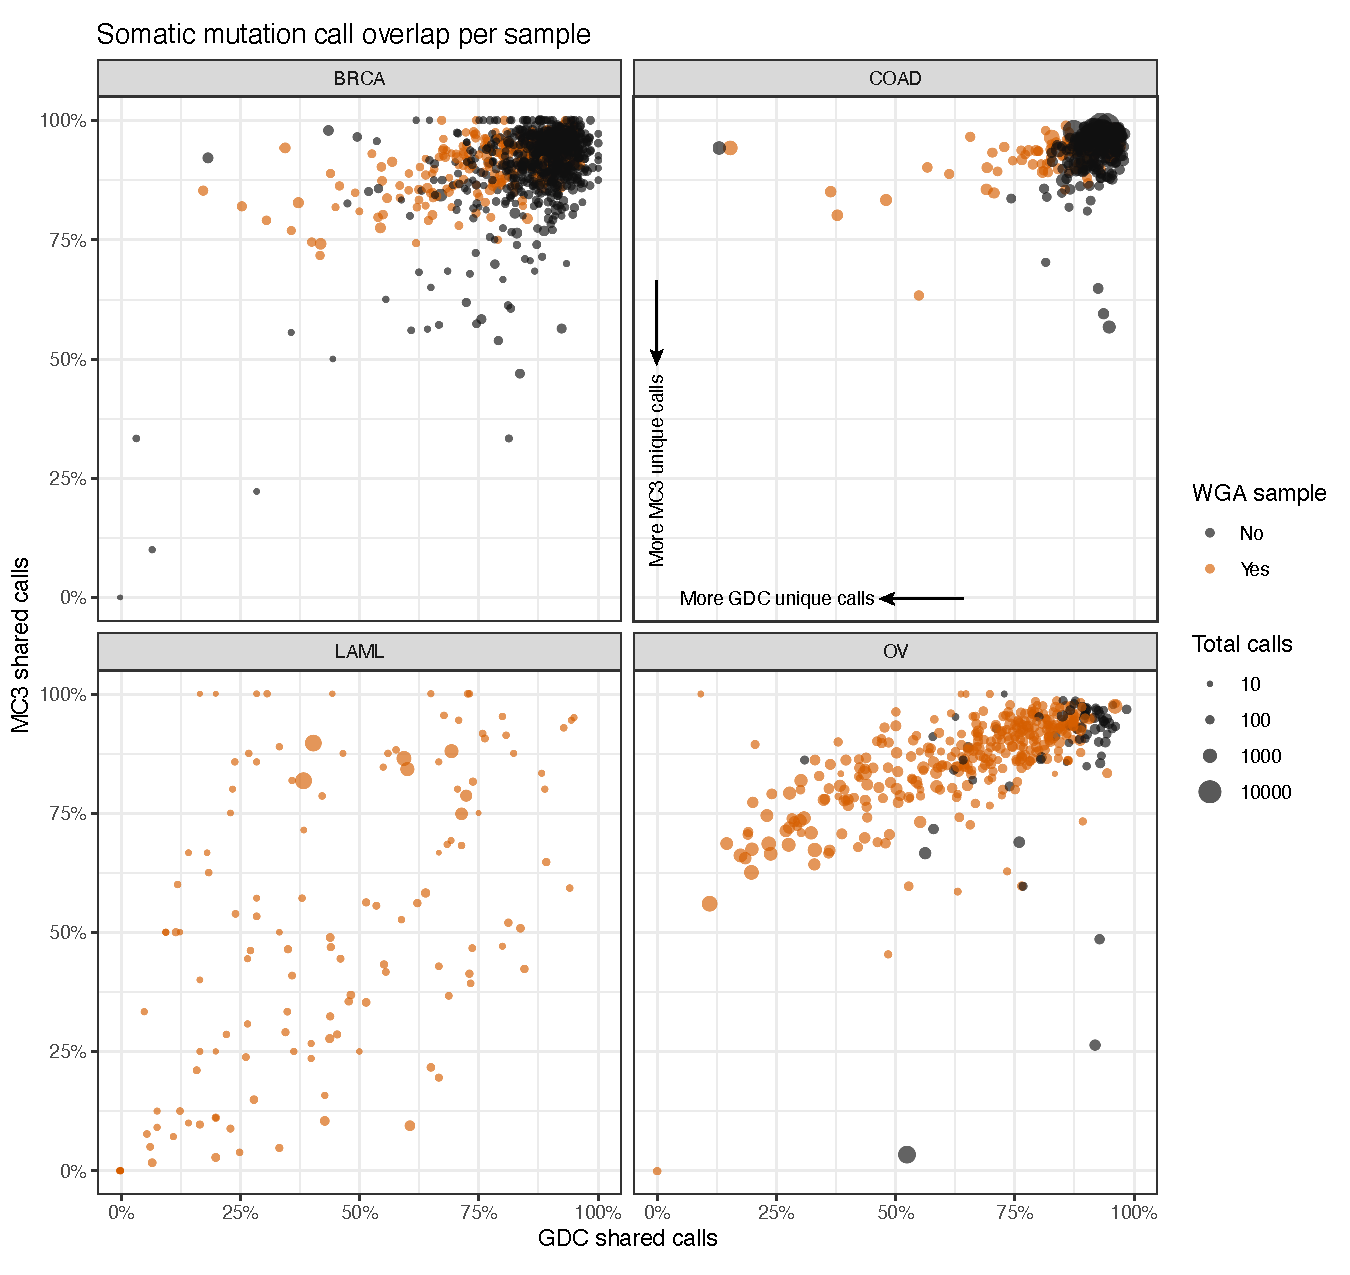
\includegraphics[width=0.8\textwidth]{figures/chap02_mutation_pipeline_qc/GDC_MC3_overlap_per_sample.pdf}
    \caption[Overlapping somatic mutation calls between GDC and MC3 per sample.]{The overlap of somatic mutation call per sample in four different cancer types. The X and Y axes represent the proportion of shared calls over the total calls from GDC and MC3 respectively. Each dot represents a sample, and the dot size indicates the numbers of somatic SNVs called. A sample has more GDC-unique or MC3-unique calls is closer to the origin. The color indicates whether WGA sequencing was employed. See also Figure S4.}
    \label{fig:mut-call-qc-overlap}
\end{figure}

From our analysis, we found that 79\% of all the public somatic mutation calls from two groups were concordant. When we excluded LAML samples, 80\% of all the public somatic calls were concordant, and the average of the fraction of concordant calls per sample improved from 72.5\% to 75.9\%. We were able to explain the remaining non-concordant public mutation calls by the three major sources of the differences (Data S5.3): for unrecoverable unique calls, mutation caller; for recoverable unique calls, filtering strategy and gene annotation version.


\section{Discussion}
The publication of the first human reference genome unleashed a torrent of cancer research, in which the field witnessed a steady transition from a largely qualitative and wet lab-based practice to one that is far more quantified and digital. While TCGA has played important catalytic and leadership roles in this transformation, the resulting increase in volume and complexity of data are pushing the limits of our capacity to store, process and make sense of it. At the same time, characterization and software technologies, analytic methods and reference data continue to rapidly evolve. The cumulative effect of these forces---size, complexity, and accelerated change---mean researchers have to confront substantial technical and logistical challenges before they can begin to ask basic biological questions.

This study helps address those challenges, and is important to the research community in several ways: (i) Scientifically, because confidence in and usability of global resources like TCGA must remain high even as the data they offer and fields they serve experience enormous growth and change. Findings published from such resources, which purport to describe fundamental biology, should remain evident no matter how the primary data are transformed after original collection; and any findings refuted after such transformations should be revised or discarded. By demonstrating significant concordance between the legacy hg19 and GDC-harmonized hg38 versions of TCGA data, our study girds the corpus of TCGA-related research and suggests it will continue to play a valuable role into the foreseeable future. (ii) Technologically, because the GDC will play an important role in the usability of many large data sets beyond TCGA---e.g. TARGET and others which are currently generating data---and in offering these data to the world the GDC has updated or introduced new data models, ontologies, back-end infrastructure as well as front-end portals and APIs. When combined with the fact that many of the scientific algorithms and knowledge bases used to generate legacy TCGA data have either evolved or been superseded, this means that the number of moving parts—and therefore the sources of potential variation—in the harmonized hg38 data served by the GDC, is high. The work reported here isolates confounding factors in the technology stack for each platform, offers sets of outliers for each platform, and indicates that TCGA results should be relatively insensitive to changes between legacy hg19 and harmonized hg38 data processing. (iii) Efficiency and cost-effectiveness, because the scope of the vetting effort reported here would be impractical for many labs or academic departments to conduct themselves prior to confidently utilizing GDC data in their work. Our study provides a framework that may guide similar comparative analyses in the future, online resources for follow-up exploration, and tools that can be hardened, generalized, and deployed to form the basis of future QC efforts in other large-scale projects.
